\documentclass{svproc}
%
% RECOMMENDED %%%%%%%%%%%%%%%%%%%%%%%%%%%%%%%%%%%%%%%%%%%%%%%%%%%
%
%%%% Standard Packages
%%<additional latex packages if required can be included here>
\usepackage{graphicx}%
\graphicspath{{./images/}}
\usepackage{multirow}%
\usepackage{amsmath,amssymb,amsfonts}%
\usepackage{mathrsfs}%
\usepackage[title]{appendix}%
% \usepackage{xcolor}%
\usepackage{textcomp}%
\usepackage{manyfoot}%
\usepackage{booktabs}%
\usepackage{algorithm}%
\usepackage{algorithmicx}%
\usepackage{algpseudocode}%
\usepackage{listings}%
\usepackage{url}
\def\UrlFont{\small\ttfamily}
% \def\UrlFont{\rmfamily}
\usepackage{footmisc}
\usepackage{multicol}
\usepackage{xurl}
\usepackage{breakurl}
\usepackage{tikz}
\usetikzlibrary{shapes,arrows,positioning}
\usepackage{subcaption}  % Add this to preamble

\setlength{\textfloatsep}{5pt plus 1pt minus 2pt}
\setlength{\intextsep}{5pt plus 1pt minus 2pt}
\setlength{\abovecaptionskip}{3pt}
\setlength{\belowcaptionskip}{3pt}

\begin{document}
\mainmatter
\title{Cognitive MRI of AI Conversations: Analyzing AI Interactions through Semantic Embedding Networks}

\titlerunning{Cognitive MRI of AI Conversations} % Abbreviated title

\author{Alex Towell \and John Matta}
\authorrunning{A. Towell et al.} % Abbreviated author list

\institute{Southern Illinois University Edwardsville,\\
Edwardsville, IL, USA\\
\email{\{atowell, jmatta\}@siue.edu}}

\maketitle

\begin{abstract}
We introduce a \emph{cognitive MRI} for AI conversations, applying network analysis to reveal thought topology hidden in linear conversation logs. We construct semantic similarity networks with user-weighted embeddings to identify knowledge communities and bridge conversations that enable cross-domain flow. Our analysis reveals heterogeneous topology: theoretical domains exhibit star-like hub structures while practical domains show tree-like hierarchies. We identify three distinct bridge types that facilitate knowledge integration across communities.
\keywords{AI conversation, complex networks, semantic embedding, conversation analysis, knowledge exploration}
\end{abstract}

\section{Introduction}

Linear conversation logs hide rich cognitive structure. We introduce a \emph{cognitive MRI} for AI conversations, using network analysis to transform linear traces into topological maps. Each conversation becomes a node in a semantic network, revealing how humans navigate knowledge domains through AI dialogue.

Our analysis of 449 ChatGPT conversations reveals heterogeneous network topology. Theoretical domains like ML/AI exhibit hub-and-spoke patterns while practical domains like programming show tree-like hierarchical structures. We identify three types of bridge conversations. Evolutionary bridges emerge through topic drift, integrative bridges deliberately synthesize concepts across domains, and pure bridges form critical links with minimal connections. These patterns suggest cognitive processes unique to conversational AI.

We build on distributed cognition \cite{hutchins1995}, which views cognitive processes as distributed across individuals and tools, and transactive memory systems \cite{wegner1987}, where groups encode, store, and retrieve knowledge collectively. In this framework, human-AI dialogue forms externalized cognitive networks where knowledge emerges through interaction, revealing the non-linear structure of thought independent of temporal sequence.

We address three research questions. First, how can we extract latent knowledge structure from conversational AI logs? Second, what network properties characterize human-AI knowledge exploration? Third, can network structure enhance navigation within personal conversation archives? Our contributions include user-weighted embeddings that prioritize human input over AI responses in a 2:1 ratio, empirical characterization revealing high modularity, and a novel taxonomy of bridge conversations with distinct structural signatures. While we analyze one author's archive, our method provides a template for multi-user studies.

\section{Related Work}

\subsection{Complex Networks in Text and Knowledge Representation}

Complex network analysis has been widely applied to textual data, from co-word occurrence networks \cite{callon1983} to citation networks \cite{price1965}. More recently, researchers have applied network science to semantic relationships, using word embeddings (dense vector representations of words that capture semantic meaning) \cite{levy2014} or document vectors \cite{mikolov2013} to create similarity-based networks.

\subsection{Semantic Embeddings for Document Representation}

Dense vector representations of text have revolutionized natural language processing. These embeddings map text to high-dimensional spaces where different dimensions encode various semantic and syntactic features. Word2Vec \cite{mikolov2013} demonstrated that word-level embeddings capture analogical relationships (e.g., king - man + woman $\approx$ queen). Modern models like \texttt{nomic-embed-text} operate at the sequence level, encoding entire conversations into vectors that capture topic, style, and semantic content simultaneously. When computing similarity between these conversation embeddings, we compare multi-faceted representations rather than simple topic matches.

\subsection{Conversation Analysis in AI Systems}

Research on analyzing conversational data with AI systems has primarily focused on dialogue structure \cite{serban2016}, user satisfaction \cite{venkatesh2018}, or topic modeling \cite{zeng2019}. Few studies have examined the network structure of conversations, particularly in the context of knowledge exploration with modern large language models. Our work extends this body of research by introducing a complex network approach to analyzing the semantic structure of AI-assisted conversations.


\section{Methods}

The code for this analysis is publicly available \cite{chatgpt-complex-net}.

\subsection{Data Collection and Preparation}

Our dataset consists of conversations conducted by a single user with ChatGPT over two years ($\approx$ 2000 conversations). We exported and preprocessed the conversations from OpenAI's ChatGPT interface to extract meaningful content while preserving conversational structure. The export process generated individual JSON files for each conversation containing both message content and metadata, establishing the foundation for our embedding generation.

\subsection{Embedding Generation}

We generated embeddings for each conversation using the \texttt{nomic-embed-text} \cite{nomicembed} model to capture semantic content while preserving topical focus despite variations in conversation length. Since users typically drive conversation direction, we weighted user inputs more heavily than AI responses when creating conversation embeddings:

\begin{enumerate}
    \item Split each conversation into user prompts and AI responses
    \item Generated embeddings for individual turns and calculated mean embeddings separately for user turns ($\vec{e}_{user}$) and AI responses ($\vec{e}_{AI}$)
    \item Created the final conversation embedding as a weighted combination:
    \begin{equation}
    \vec{e}_{conversation} = \frac{2 \times \vec{e}_{user} + \vec{e}_{AI}}{\|2 \times \vec{e}_{user} + \vec{e}_{AI}\|}
    \end{equation}
\end{enumerate}

We selected a 2:1 weighting ratio to prioritize user intent while still incorporating AI contributions. This choice reflects our assumption that user prompts better represent the conversation's semantic focus than AI responses, which tend to be lengthier and more elaborative. Unit normalization preserves relative semantic relationships regardless of conversation length.

% INTEGRATED ABLATION STUDY SECTION
% Replace sections 3.3, 3.4, and parts of 4.2 with this comprehensive analysis

\subsection{Comprehensive Ablation Study}

To validate our methodological choices and understand their impact on network structure, we conducted an extensive ablation study examining 63 parameter configurations. This analysis reveals how embedding weights and similarity thresholds jointly determine both quantitative network properties and qualitative knowledge organization.

\subsubsection{Experimental Design}

We performed a complete 2D parameter sweep examining:
\begin{itemize}
    \item \textbf{Nine weight ratios}: 100:1, 4:1, 2:1, 1.618:1, 1:1, 1:1.618, 1:2, 1:4, 1:100 (user:AI)
    \item \textbf{Seven similarity thresholds}: 0.8, 0.825, 0.85, 0.875, 0.9, 0.925, 0.95
\end{itemize}

For each configuration, we reconstructed the complete network, detected communities using the Louvain method, and analyzed both structural metrics and semantic coherence.

\subsubsection{Phase Transition and Critical Threshold}

\begin{figure}[h]
\centering
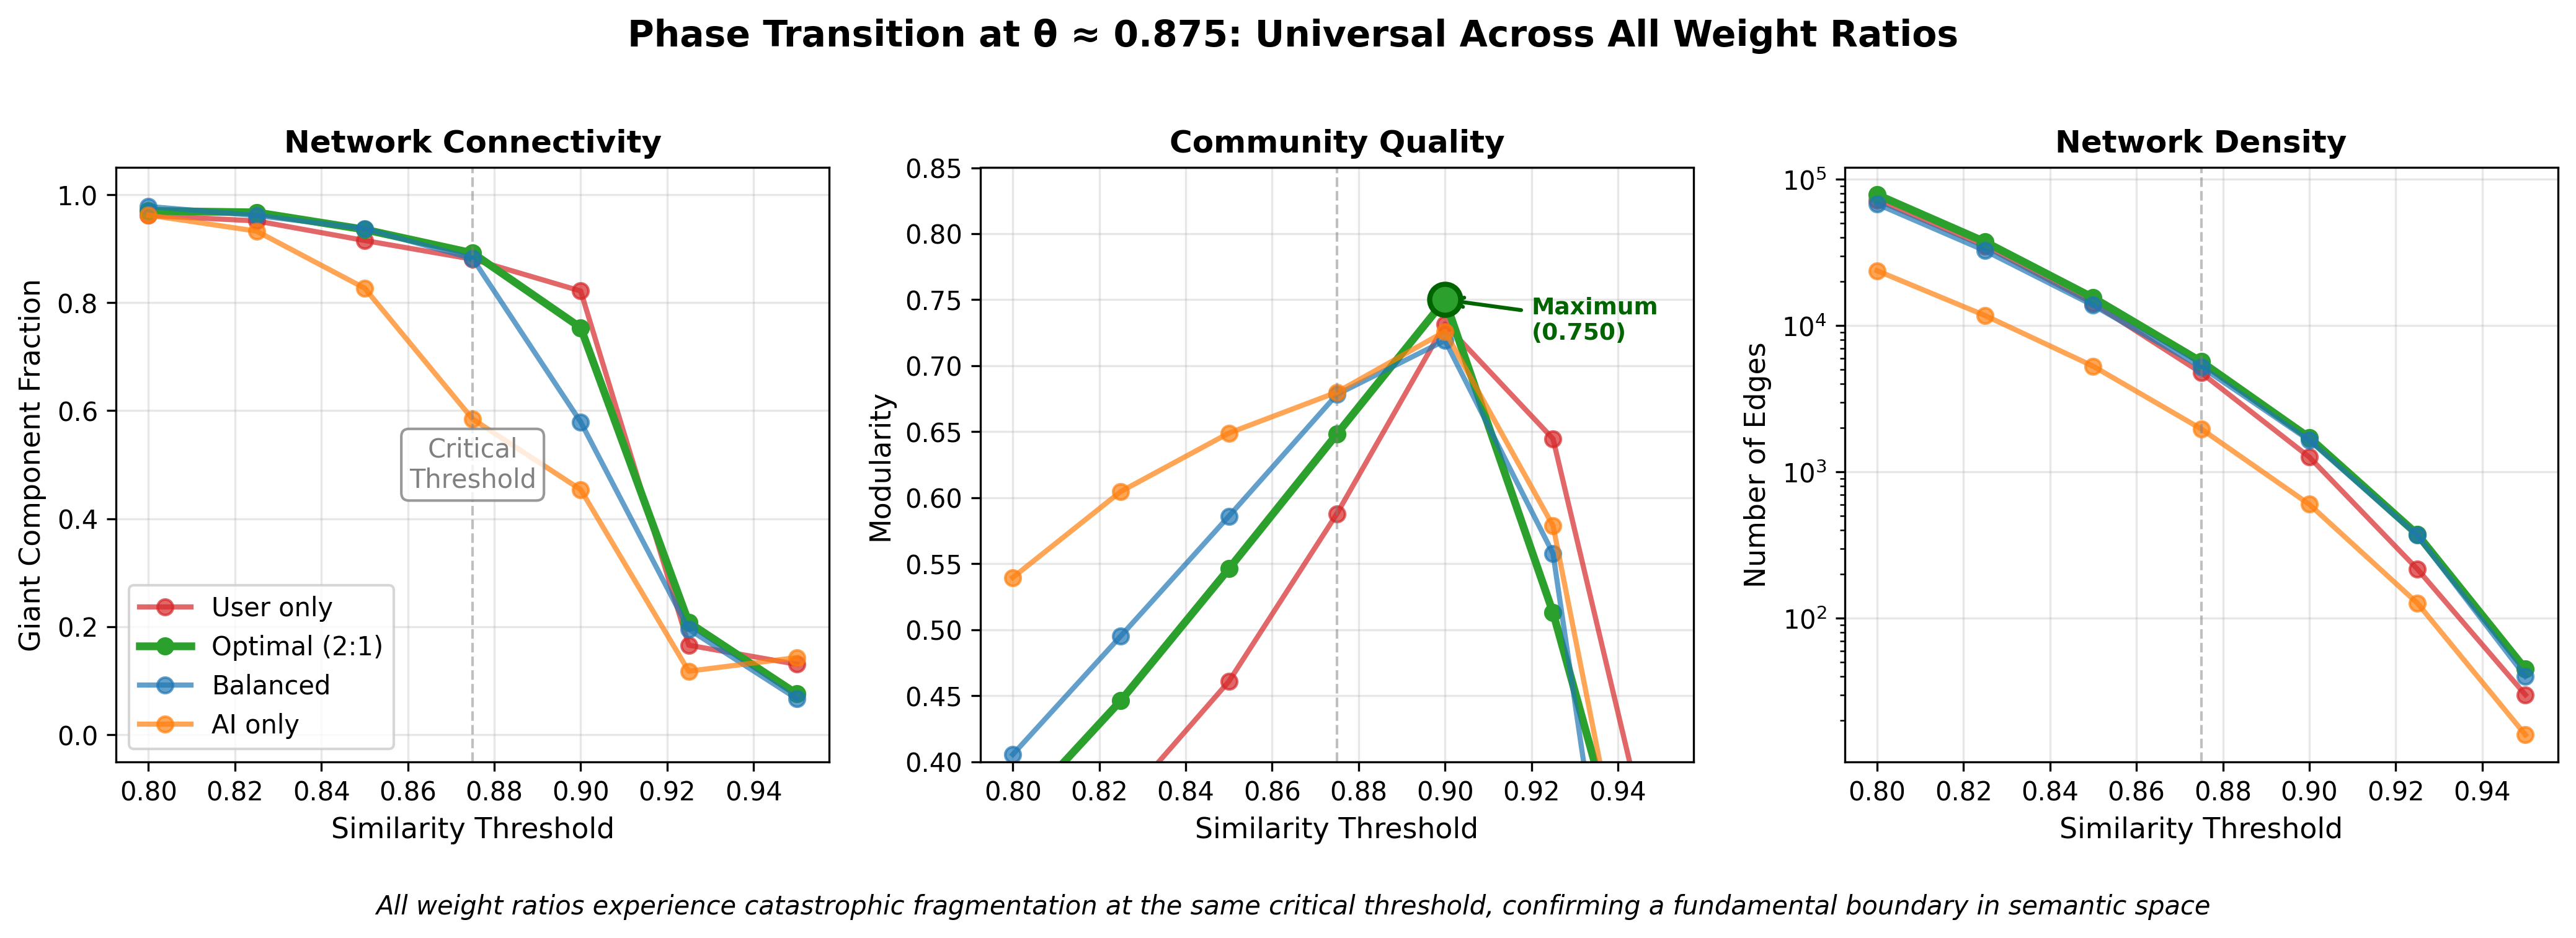
\includegraphics[width=\textwidth]{./images/threshold_evolution_clean.png}
\caption{Network metrics across similarity thresholds showing universal phase transition at $\theta \approx 0.875$ independent of weight ratio.}
\label{fig:phase_transition}
\end{figure}

Figure~\ref{fig:phase_transition} reveals a critical phase transition at similarity threshold $\theta \approx 0.875$. Below this threshold, the network maintains $>90\%$ connectivity; above it, catastrophic fragmentation occurs. This percolation phenomenon is remarkably consistent across all weight ratios, suggesting a fundamental boundary in semantic coherence.

\begin{table}[h]
\centering
\caption{Network Properties at Critical Thresholds (2:1 Weight Ratio)}
\label{tab:threshold_critical}
\begin{tabular}{lccccc}
\toprule
\textbf{Threshold} & \textbf{Nodes} & \textbf{Edges} & \textbf{Giant Comp.} & \textbf{Modularity} & \textbf{Communities} \\
\midrule
0.850 & 1,210 & 15,523 & 93.6\% & 0.546 & 13 \\
0.875 & 934 & 5,675 & 89.2\% & 0.648 & 15 \\
\textbf{0.900} & \textbf{449} & \textbf{1,615} & \textbf{75.4\%} & \textbf{0.750} & \textbf{15} \\
0.925 & 284 & 375 & 20.8\% & 0.513 & 5 \\
\bottomrule
\end{tabular}
\end{table}


\subsubsection{Optimal Weight Ratio Determination}

\begin{figure}[h]
\centering
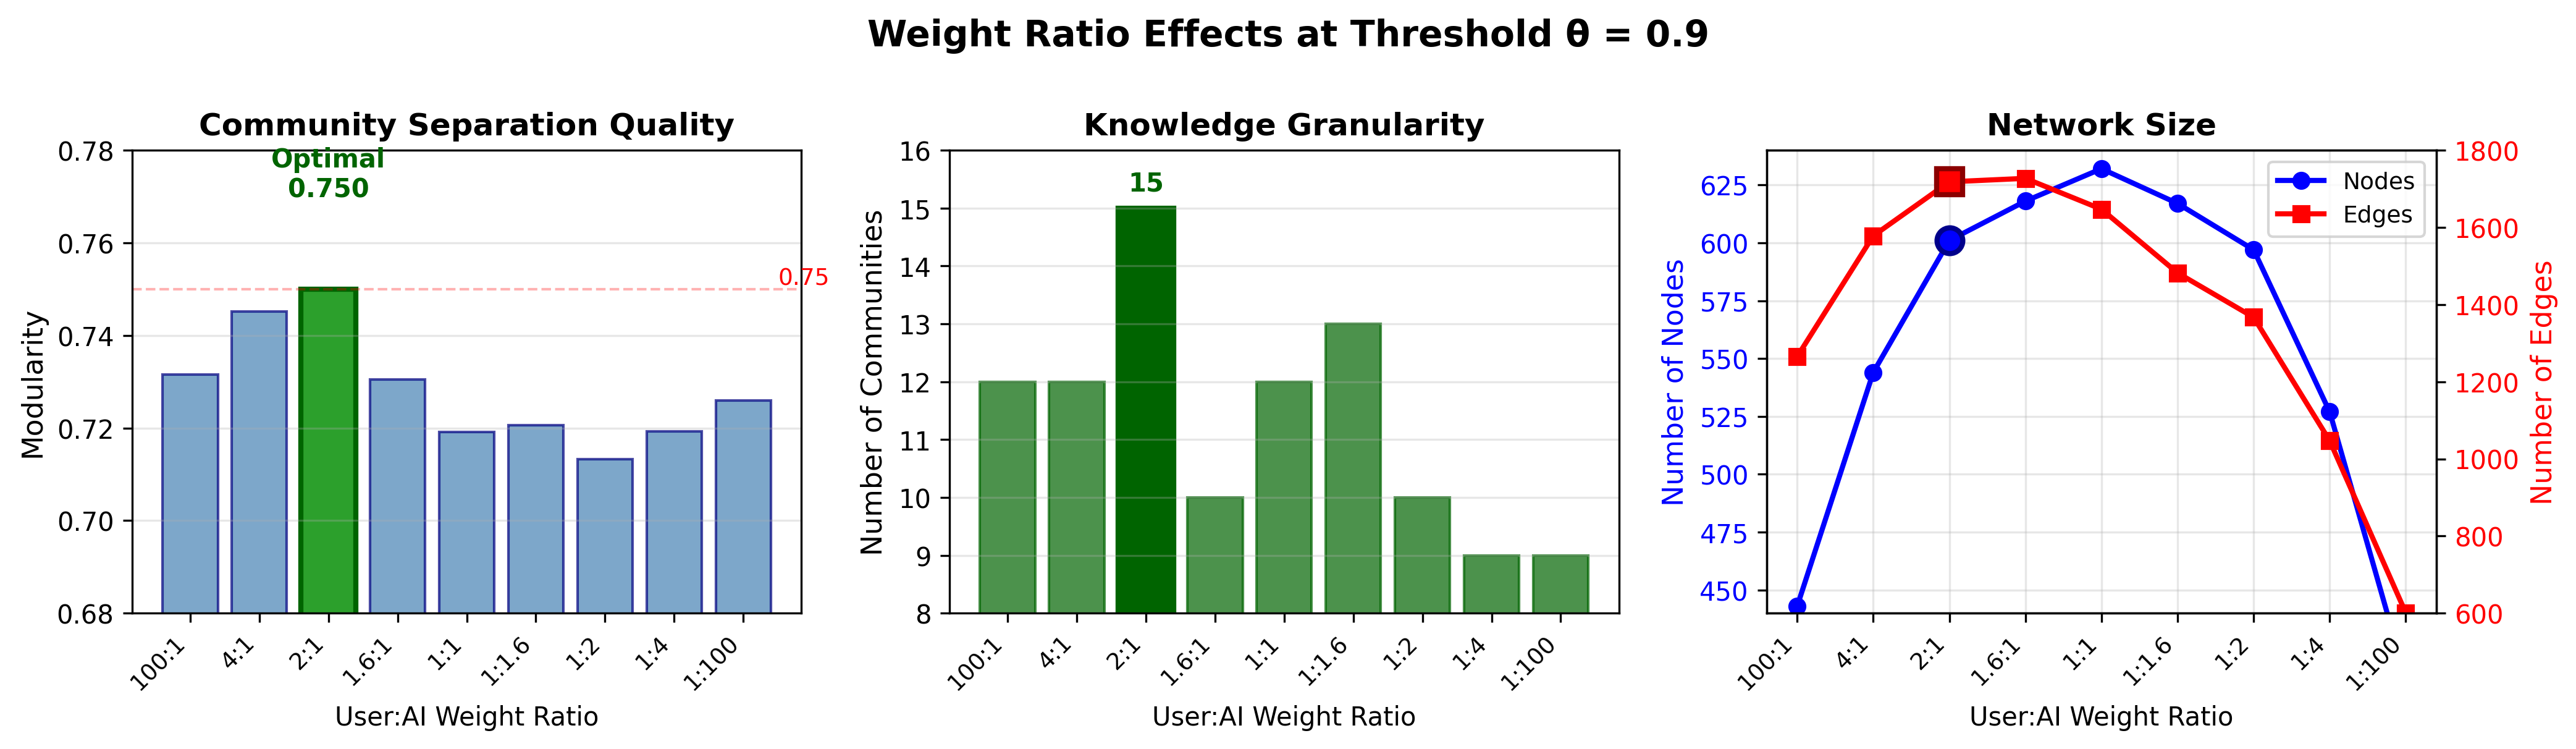
\includegraphics[width=\textwidth]{./images/weight_ratio_analysis_clean.png}
\caption{Weight ratio optimization at $\theta = 0.9$. The 2:1 user:AI ratio maximizes modularity (0.750) while maintaining 15 distinct communities.}
\label{fig:weight_ratio_analysis}
\end{figure}

At our chosen threshold of 0.9, systematic variation of weight ratios reveals that the 2:1 user:AI configuration maximizes modularity (0.750) while preserving network coherence. Figure~\ref{fig:weight_ratio_analysis} demonstrates how this ratio achieves optimal balance across multiple metrics.

\subsubsection{Knowledge Organization Across Weight Ratios}

While weight ratios affect modularity optimization, our analysis reveals that the underlying topic distribution remains remarkably stable across configurations (ML/AI: 26-37\%, General topics: 47-55\%). This stability suggests that knowledge domains are inherent to the conversation content rather than imposed by weighting schemes. 

The 2:1 user:AI ratio proves optimal precisely because it maximizes modularity (0.750) without distorting this natural topic structure. At this ratio, we observe 15 well-defined communities that preserve topic focus while incorporating semantic breadth from AI responses. User-heavy ratios (100:1, 4:1) create overly fragmented communities that separate related concepts, while AI-heavy ratios (1:4, 1:100) merge distinct domains based on response patterns rather than knowledge structure.

\subsubsection{Case Study: Semantic Boundaries at the Phase Transition}

The phase transition at $\theta = 0.875$ reveals more than statistical fragmentation—it exposes semantic boundaries between distinct conversational contexts, as illustrated in Figure~\ref{fig:semantic_boundary}:

\begin{figure}[h]
\centering
\begin{subfigure}{0.48\textwidth}
    \centering
    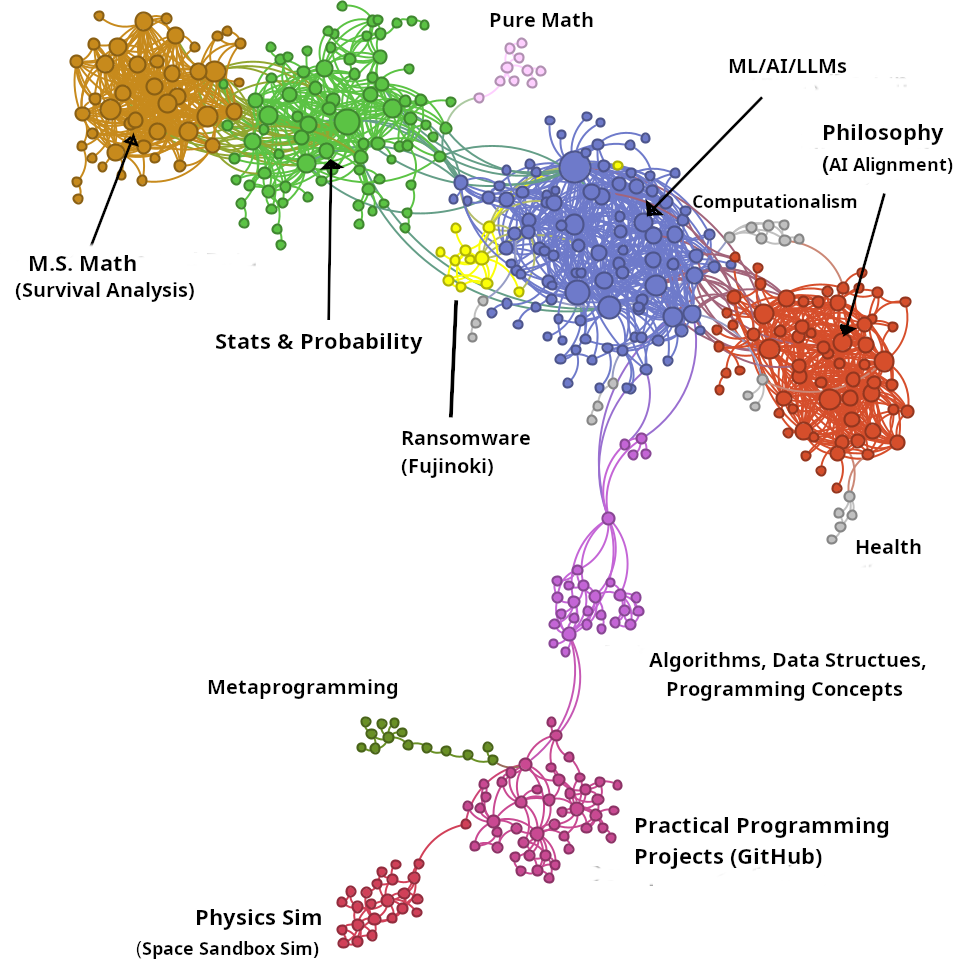
\includegraphics[width=\textwidth]{./images/cluster-vis-topics-better.png}
    \caption{$\theta=0.9$: Distinct contexts separated}
\end{subfigure}
\hfill
\begin{subfigure}{0.48\textwidth}
    \centering
    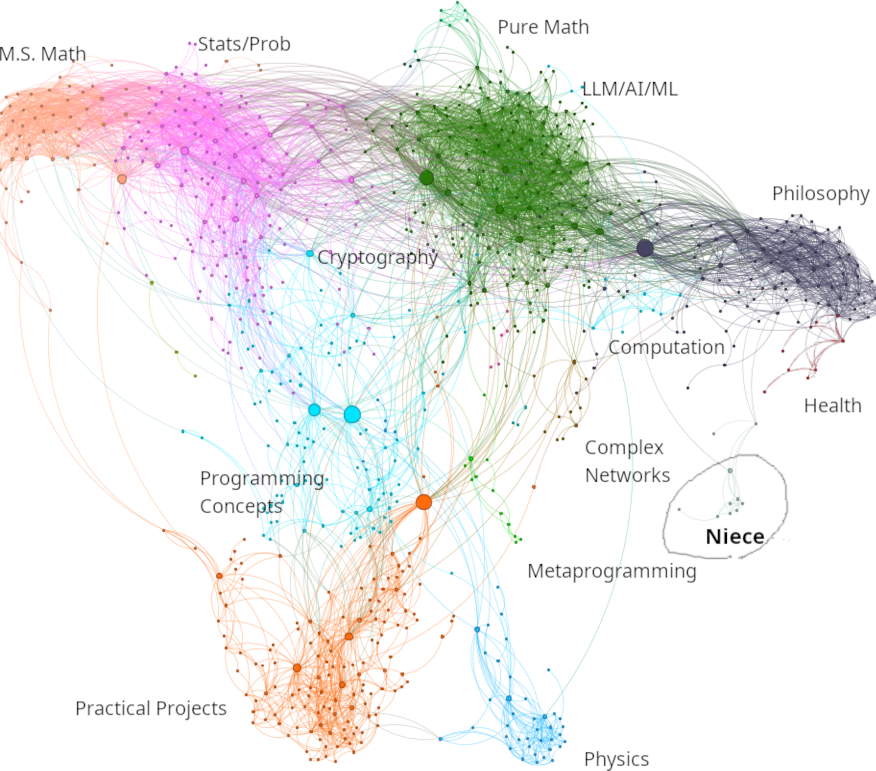
\includegraphics[width=\textwidth]{./images/0.875-wild-better.png}
    \caption{$\theta=0.875$: Peripheral context emerges}
\end{subfigure}
\caption{Semantic boundaries revealed by threshold variation. Niece conversations remain isolated at $\theta=0.9$ (left) but connect through philosophical bridges at $\theta=0.875$ (right).}
\label{fig:semantic_boundary}
\end{figure}

As shown in Figure~\ref{fig:semantic_boundary}, conversations with the author's 13-year-old niece—characterized by artistic topics, informal language, and creative storytelling—remain isolated at threshold 0.9 (left panel) but connect to the giant component at 0.875 (right panel) through philosophical bridge conversations. This 2.5\% difference in similarity threshold captures the semantic distance between:

\begin{itemize}
    \item Primary knowledge network: Technical vocabulary, formal register, domain expertise
    \item Peripheral context: Age-appropriate explanations, creative topics, informal style
\end{itemize}

This validates our threshold selection: $\theta=0.9$ preserves analytical clarity by maintaining natural boundaries between cognitive contexts.

\subsubsection{Parameter Selection Justification}

Our comprehensive ablation study confirms the optimality of threshold 0.9 with 2:1 user:AI weighting:

\begin{enumerate}
    \item \textbf{Maximum modularity} (0.750) ensures clear community boundaries
    \item \textbf{Post-transition operation} removes noise while preserving essential connections (1,615 edges from ~100K possible)
    \item \textbf{Semantic coherence} maintains topic-focused communities reflecting human knowledge organization
    \item \textbf{Boundary preservation} separates distinct conversational contexts while revealing their connection points
\end{enumerate}

\begin{table}[h]
\centering
\caption{2D Parameter Sweep Heatmap Summary}
\label{tab:2d_summary}
\begin{tabular}{lccccc}
\toprule
\textbf{Metric} & \textbf{Primary Driver} & \textbf{Secondary Effect} & \textbf{Optimal Config} \\
\midrule
Giant Component & Threshold & None & $\theta \leq 0.875$ \\
Modularity & Both & Weight ratio modulates & 2:1 at $\theta=0.9$ \\
Clustering & Weight ratio & Threshold modulates & User-heavy ratios \\
Density & Threshold & None & Application-dependent \\
Topic Coherence & Weight ratio & N/A & 2:1 to 4:1 \\
\bottomrule
\end{tabular}
\end{table}

The independence of threshold effects (controlling connectivity) from weight ratio effects (controlling organization) suggests these parameters tune orthogonal aspects of network structure. Threshold acts as a \emph{semantic filter} determining which connections exist, while weight ratio provides \emph{semantic perspective} determining how knowledge organizes within the connected structure.

Using this network representation, we applied several standard complex network analysis techniques to characterize its structure. We used the Louvain method \cite{blondel2008} for community detection to identify distinct knowledge domains and calculated various centrality measures (degree, betweenness, hub) to identify significant nodes in the network. We also examined core-periphery structure to understand topic stratification.

Betweenness centrality identified bridge conversations that facilitate inter-community knowledge transfer where separate domains integrate (Section~\ref{community_structure}).

\section{Results}

\subsection{Knowledge Domain Organization}

The network reveals rich topological structure, spontaneously organizing into thematic clusters despite no explicit categorization. Figure~\ref{fig:network_vis} shows striking heterogeneity: mathematical and ML communities (\emph{M.S. Math}, \emph{Stats \& Probability}, \emph{ML/AI/LLMs}, \emph{Philosophy}) exhibit dense hub-and-spoke structures with dominant central nodes characteristic of scale-free networks. In contrast, other communities show different organization: \emph{Metaprogramming} displays tree-like branching, while \emph{Practical Programming Projects} and \emph{Computationalism} show more dispersed structures without dominant hubs. Specialized bridge nodes facilitate cross-domain transfer between these communities.

\begin{figure}[t]
\centering
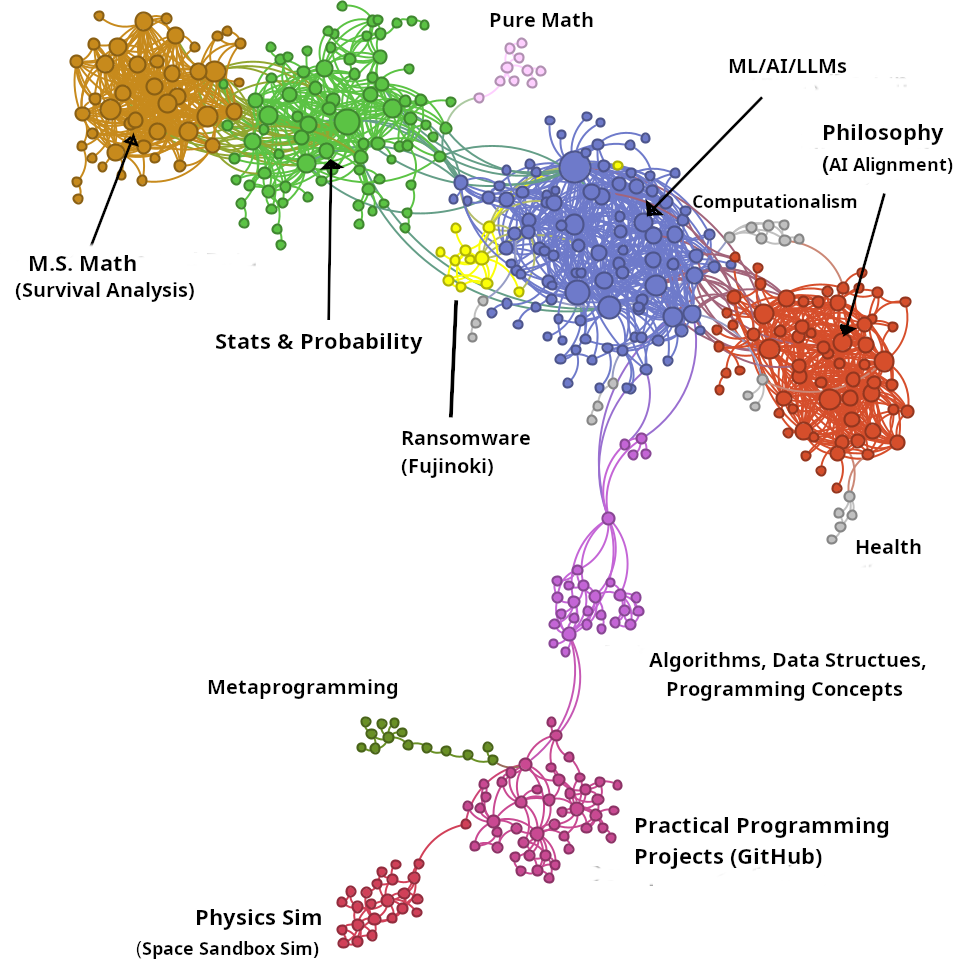
\includegraphics[width=4.5in]{./images/cluster-vis-topics-better.png}
\caption{Giant component at 0.9 threshold showing 15 distinct communities.}
\label{fig:network_vis}
\end{figure}

The network comprises 449 nodes and 1615 edges with average degree 7.19, clustering coefficient 0.60, and average path length 5.81. These metrics reveal strong local clustering with relatively long path lengths, indicating ``cognitive distance'' when navigating between knowledge domains. Such organization likely reflects cognitive constraints on knowledge exploration, where conceptual bridges are necessary to move between specialized domains.

 

\subsection{Degree Distribution and Network Structure}

Figure \ref{fig:degree_hist} shows the degree histogram for our conversation network. The strongly right-skewed distribution reveals that while the majority of conversations maintain connections with only a few semantically similar conversations, a small number of hub conversations exhibit substantially higher degrees. This pattern markedly contrasts with the bell-shaped distributions typical of random networks, indicating non-random organizational principles.

\begin{figure}[!htbp]
\centering
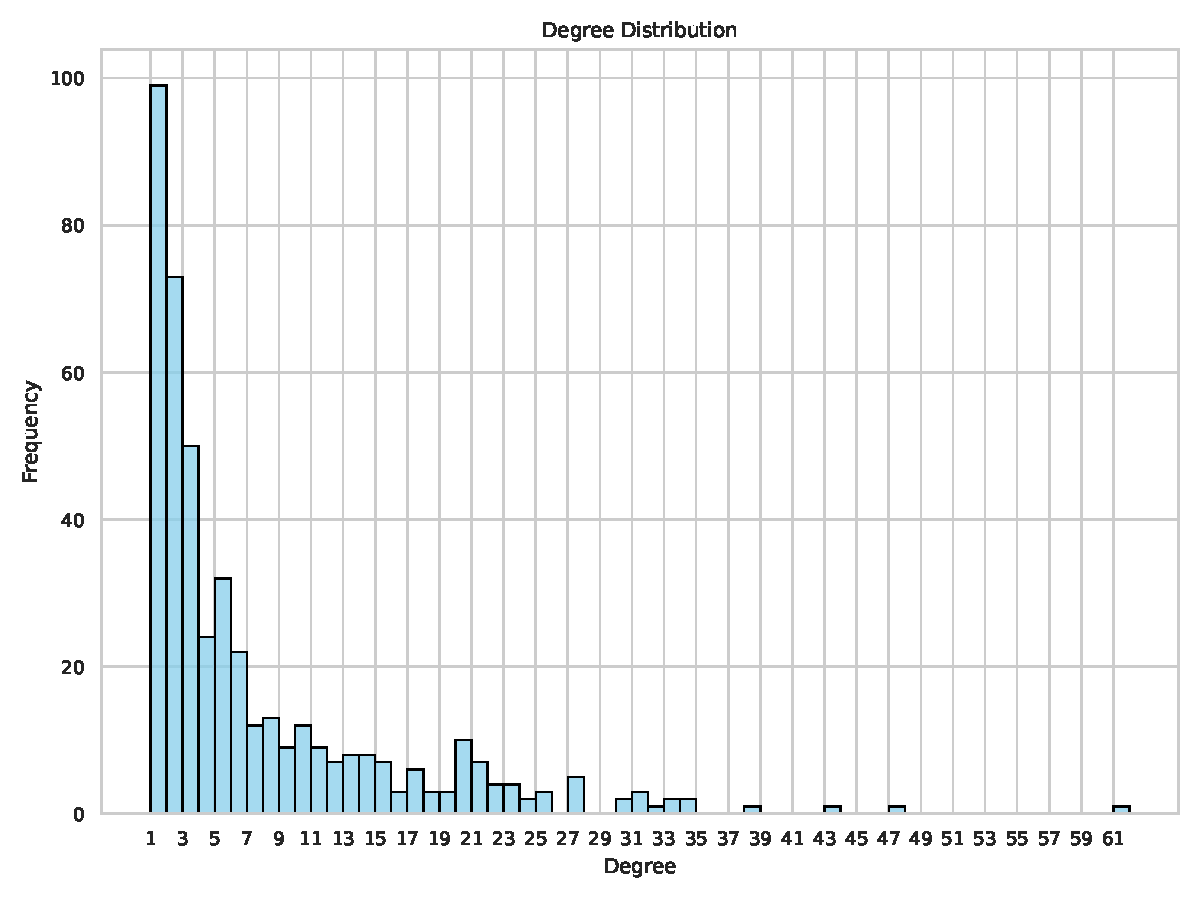
\includegraphics[width=3.5in]{./images/degree_distribution_histogram.pdf}
\caption{Degree distribution of the conversation network, showing characteristic right-skewed pattern.}
\label{fig:degree_hist}
\end{figure}

Comparing our network structure with scale-free networks generated by preferential attachment reveals important differences. As visible in Figure~\ref{fig:network_vis}, our network exhibits significantly higher clustering and path length than standard scale-free networks. These deviations stem from the network's cognitive organization. Many communities display elongated, tree-like structures rather than the star-like configurations typical of pure preferential attachment. This is particularly evident in specialized knowledge domains like \emph{Programming Projects}, where conversations tend to be independent and focused on specific topics rather than forming clusters of related conversations.

This suggests evolution beyond preferential attachment, reflecting cognitive exploration with hub formation limited by specialization and cross-domain constraints. Additionally, the network exhibits core-periphery organization with 25.6\% of conversations forming a densely connected core (average degree: 18.94) surrounded by a sparser periphery (average degree: 3.15), indicating stratification between general and specialized topics.

\subsection{Community Structure}
\label{community_structure}

Louvain detection revealed 15 communities representing thematically coherent domains. Table~\ref{tab:communities} presents the five largest, where Core \% indicates k-core membership \cite{seidman1983} and Clustering shows average local coefficients.

\begin{table}
\centering
\caption{Major Community Characteristics}
\label{tab:communities}
\begin{tabular}{cccccl}
\toprule
\textbf{Comm.} & \textbf{Size} & \textbf{Avg. Degree} & \textbf{Core \%} & \textbf{Clustering} & \textbf{Primary Topic} \\
\midrule
3 & 103 & 8.60 & 31.1\% & 0.465 & ML/AI/LLM (23\%) \\
12 & 82 & 7.09 & 24.4\% & 0.405 & Stats \& Probability (18\%) \\
7 & 65 & 10.03 & 44.6\% & 0.531 & Philosophy \& AI Ethics (14\%) \\
14 & 44 & 13.45 & 59.1\% & 0.576 & M.S. Math/Analysis (10\%) \\
6 & 45 & 3.78 & 8.9\% & 0.396 & Programming Projects (10\%) \\
\bottomrule
\end{tabular}
\end{table}

Communities correspond to distinct knowledge domains: Community 3 (\emph{ML/AI/LLM}) covers AI architectures and training; Community 12 (\emph{Stats \& Probability}) encompasses statistical inference and modeling; Community 7 (\emph{Philosophy \& AI Ethics}) addresses consciousness and AI alignment; Community 14 (\emph{M.S. Math/Analysis}) contains graduate-level mathematical analysis; Community 6 (\emph{Programming Projects}) focuses on practical implementation.

The variation in internal structure (average degree, clustering, and core percentage) suggests different conversation patterns across domains. For example, community 14 shows characteristics of a specialized knowledge domain with dense expert connections, while community 6 resembles a more practical, service-oriented domain with mostly peripheral connections.

\subsection{Bridges and Hubs: Dual Roles in Knowledge Integration}

Analysis of centrality measures reveals conversations serving dual roles as bridges (high betweenness) and hubs (high degree). Table~\ref{tab:bridges} presents the top conversations ranked by betweenness centrality.

\begin{table}
\centering
\caption{Top Bridge Conversations}
\label{tab:bridges}
\begin{tabular}{lrr}
\toprule
\textbf{Conversation} & \textbf{Betweenness} & \textbf{Degree} \\
\midrule
\url{geometric-mean-calculation} & 45467.51 & 61 \\
\url{mcts-code-analysis-suggestions} & 36909.13 & 10 \\
\url{loss-in-llm-training} & 35118.59 & 30 \\
\url{algotree-generate-unit-tests-flattree} & 31869.77 & 13 \\
\url{compile-cuda-program-linux} & 9775.00 & 2 \\
\bottomrule
\end{tabular}
\end{table}

Three distinct bridge types emerge, extending structural bridge classifications \cite{granovetter1973,burt1992} with semantic characterization. First, \textbf{evolutionary bridges} are high-degree nodes that expand across domains through topic drift. For example, \url{geometric-mean-calculation} evolved from geometric means into probability theory, neural networks, and tokenization (degree=61, betweenness=45467). Second, \textbf{integrative bridges} are moderate-degree nodes that deliberately synthesize domains, such as \url{mcts-code-analysis-suggestions} which integrates AI theory with software engineering (degree=10, betweenness=36909). Third, \textbf{pure bridges} are low-degree critical links like \url{compile-cuda-program-linux} (degree=2, betweenness=9775).

\begin{figure}[!h] %tbp]
\centering
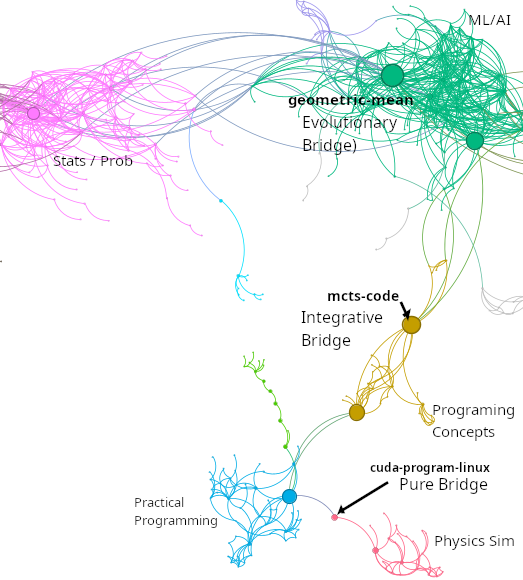
\includegraphics[width=3.5in]{./images/bridge-better.png}
\caption{Bridge conversations connecting knowledge communities (blue: ML/AI/LLM, purple: Programming Projects).}
\label{fig:bridge_zoom}
\end{figure}

Figure~\ref{fig:bridge_zoom} illustrates these distinct bridging mechanisms in the network structure.

Notably, some conversations like \url{geometric-mean-calculation} function as both bridges and hubs, while others like \url{mle-bootstrapping-simulation} (degree=47) serve primarily as within-community hubs. Hub nodes exhibit lower clustering coefficients (0.224 vs 0.436 average), creating ``star-like'' structures that position them as conceptual distribution points. The concentration of hubs in community 3 (\emph{ML/AI/LLM}) suggests this domain serves as a conceptual anchor, contrasting with the distributed organization in practical domains like \emph{Programming Projects}. These patterns reveal how conversation networks follow unique evolutionary dynamics.

\section{Discussion and Conclusion}

\subsection{Cognitive Interpretation}

The network reveals cognitive patterns distinct from academic citation networks, which provide a natural comparison as both capture knowledge exploration processes. While citation networks evolve through preferential attachment with papers citing influential work (creating major hubs like foundational papers with thousands of citations), conversation networks reflect real-time cognitive exploration. Our finding of heterogeneous topology with some tree-like, branching clusters entirely lacking hubs contrasts sharply with citation networks' consistent scale-free structure. In citation networks, even specialized subfields connect to seminal papers, but our conversational communities like \emph{Metaprogramming} show purely branching exploration without central authorities. This suggests cognitive exploration follows different organizing principles: intense local exploration punctuated by cross-topic jumps rather than cumulative authority building. This forms a \emph{structural trace of thinking}. Just as an MRI reveals the physical structure of the brain, this cognitive MRI reveals the topological structure of thought preserved in conversation logs. Three community types emerge. \emph{Expert domains} like Stats/Probability are densely connected with high clustering. \emph{Bridging domains} like ML/AI/LLM are broadly connected with lower clustering. \emph{Task domains} like Programming are sparsely connected and implementation-focused. This suggests design implications: surfacing pure bridges could facilitate creative leaps, while respecting natural knowledge boundaries could improve retrieval systems.

\subsection{Limitations and Future Work}

Our single-user study limits generalizability; future work should analyze diverse users to understand how cognitive styles influence exploration patterns. The static snapshot could be extended using temporal metadata to reveal how knowledge domains evolve through continued AI interaction.

\subsection{Conclusion}

We presented a novel application of complex network analysis to AI conversations, revealing distinct knowledge communities and bridge conversations. The heterogeneous network topology reflects cognitive processes in topic exploration, with bridges facilitating movement between specialized domains. This \emph{cognitive MRI} methodology provides a framework for understanding and enhancing AI-assisted knowledge work as these systems become increasingly integrated into human cognition.

\bibliographystyle{splncs04}
\begin{thebibliography}{00}

\bibitem{callon1983} M. Callon, J.-P. Courtial, W. A. Turner, and S. Bauin, "From translations to problematic networks: An introduction to co-word analysis," Social Science Information, vol. 22, no. 2, pp. 191-235, 1983.

\bibitem{devlin2019} J. Devlin, M.-W. Chang, K. Lee, and K. Toutanova, "BERT: Pre-training of deep bidirectional transformers for language understanding," in Proc. NAACL-HLT, 2019.

\bibitem{hutchins1995} E. Hutchins, \emph{Cognition in the Wild}. Cambridge, MA: MIT Press, 1995.

\bibitem{levy2014} O. Levy and Y. Goldberg, "Neural word embedding as implicit matrix factorization," in Advances in Neural Information Processing Systems, 2014.

\bibitem{mikolov2013} T. Mikolov, I. Sutskever, K. Chen, G. S. Corrado, and J. Dean, "Distributed representations of words and phrases and their compositionality," in Advances in Neural Information Processing Systems, 2013.

\bibitem{pennington2014} J. Pennington, R. Socher, and C. D. Manning, "GloVe: Global vectors for word representation," in Proc. EMNLP, 2014.

\bibitem{price1965} D. J. de S. Price, "Networks of scientific papers," Science, vol. 149, no. 3683, pp. 510-515, 1965.

\bibitem{serban2016} I. V. Serban, R. Lowe, P. Henderson, L. Charlin, and J. Pineau, "A survey of available corpora for building data-driven dialogue systems," arXiv preprint arXiv:1512.05742, 2016.

\bibitem{venkatesh2018} A. Venkatesh et al., "On evaluating and comparing conversational agents," arXiv preprint arXiv:1801.03625, 2018.

\bibitem{wegner1987} D. M. Wegner, "Transactive memory: A contemporary analysis of the group mind," in \emph{Theories of Group Behavior}, pp. 185-208, Springer, 1987.

\bibitem{zeng2019} Z. Zeng, H. Deng, X. Guo, and H. Wang, "Topic modeling for short texts with insider and outsider word separation," in Proc. IEEE Int. Conf. on Big Data, 2019.

\bibitem{chatgpt-complex-net} A. Towell, "chatgpt-complex-net: Complex network analysis of ChatGPT conversations," 2025. [Online]. Available: \url{https://github.com/queelius/chatgpt-complex-net}. DOI: \url{https://doi.org/10.5281/zenodo.15314235}

\bibitem{nomicembed} Z. Nussbaum, J. X. Morris, B. Duderstadt, and A. Mulyar, "Nomic Embed: Training a Reproducible Long Context Text Embedder," arXiv preprint arXiv:2402.01613, 2025.

\bibitem{blondel2008} V. D. Blondel, J.-L. Guillaume, R. Lambiotte, and E. Lefebvre, "Fast unfolding of communities in large networks," Journal of Statistical Mechanics: Theory and Experiment, vol. 2008, no. 10, p. P10008, 2008.

\bibitem{seidman1983} S. B. Seidman, "Network structure and minimum degree," Social Networks, vol. 5, no. 3, pp. 269-287, 1983.

\bibitem{granovetter1973} M. S. Granovetter, "The strength of weak ties," American Journal of Sociology, vol. 78, no. 6, pp. 1360-1380, 1973.

\bibitem{burt1992} R. S. Burt, \emph{Structural Holes: The Social Structure of Competition}. Cambridge, MA: Harvard University Press, 1992.

\end{thebibliography}

\end{document}



